\documentclass{letnab}
\pagestyle{fancy}
\usepackage{tabu}
\usepackage{units}
\usepackage{lscape}
\usepackage{ctable} % for \specialrule command

\usepackage{booktabs}
\rhead{Общая физика МФТИ}
\lhead{Лабораторная работа 2.3.1} 

\renewcommand{\headrulewidth}{2pt}
\begin{document}

	\begin{titlepage}
		
		
		
		\center % Center everything on the page
		
		
		
		%----------------------------------------------------------------------------------------
		%	HEADING SECTIONS
		%----------------------------------------------------------------------------------------
		
		\textsc{\LARGE Московский Физико-Технический Институт}\\[1,5cm] % Name of your university/college
		% Major heading such as course name
		\textsc{\Large Кафедра общей физики}\\[0.5cm]
		\textsc{\large Отчет о выполнении лабораторной работы \textnumero  2.1.1}\\[0.5cm] % Minor heading such as course title
		
		%----------------------------------------------------------------------------------------
		%	TITLE SECTION
		%----------------------------------------------------------------------------------------
		
		\HRule
		\\[0.4cm]
		{ \huge \bfseries Измерение удельной теплоёмкости воздуха при постоянном давлении}
		\\[0.2cm] % Title of your document
		\HRule
		\\[1.5cm]
		
		
		
		%----------------------------------------------------------------------------------------
		%	AUTHOR SECTION
		%----------------------------------------------------------------------------------------
		
		\begin{minipage}{0.7\textwidth}
			\begin{center} \large
				\emph{Автор:} Алексей \textsf{Домрачев} 615 группа
			\end{center}
		\end{minipage}
		\\[1.0cm]
		\begin{minipage}{0.9\textwidth}
			\begin{center} \large
				\emph{Преподаватель:} Александр Дмитриевич \textsf{Калашников} % Supervisor's Name
			\end{center}
		\end{minipage}
		\vfill 
	%	\begin{bottompar}
			
\includegraphics[width = 80 mm]{logo.png}	\\[1,0cm]
			{\large \today}
	%	\end{bottompar}
		% Fill the rest of the page with whitespace
		
	\end{titlepage}



\paragraph{Цель работы:}Измерение объёмов форвакуумной и высоковакуумной частей установки;  определение скорости откачки системы в стационарном режиме, а также по ухудшению и улучшению вакуума.
\paragraph{В работе используются:}Вакуумная установка с манометрами: масляным, термопарным и ионизационным.
\paragraph{Теория.} 
С физической точки зрения низкий вакуум переходит в высокий, когда длина свободного пробега молекул становится сравнимой с размером установки (а течение газа сугубо молекулярным); сверхвысокий вакуум характерен важностью процессов адсорбции и десорбции частиц на поверхности вакуумной камеры.\\
В этой работе изучаются традиционные методы откачки механическим форвакуумным насосом до давления $10^{-2}$ торр и диффузионным масляным насосом до $10^{-5}$ торр, а также методы измерения вакуума в этом диапазоне\\
\paragraph{Рабочие формулы.}
Объёмы частей установки будем рассчитывать с помощью закона Бойля--Мариотта для идеального газа: $PV=const$ \\
Обозначим через $Q_\text{д}$ количество газа, десорбирующегося с поверхности откачиваемого объема в единицу времени, через $Q_\text{и}$ — количество газа, проникающего в единицу времени в этот объем извне --- через течи. Будем считать, что насос обладает скоростью откачки $W$ и в то же время сам является источником газа; пусть $Q_\text{н}$ --- поток газа, поступающего из насоса назад в откачиваемую систему. Будем измерять количество газа $Q_\text{д},\, Q_\text{н}$ и $Q_\text{и}$ в единицах $PV$ (легко видеть, что это произведение с точностью до множителя $RT/\mu$ равно массе газа). Основное уравнение, описывающее процесс откачки, имеет вид 
\begin{equation}
-VdP=(PW-Q_\text{д}-Q_\text{н} - Q_\text{и})dt.
\end{equation}
Левая часть этого уравнения равна убыли газа в откачиваемом
объеме $V$ , а правая определяет количество газа, уносимого насосом,
и количество прибывающего вследствие перечисленных выше причин
за время $dt$. При достижении предельного вакуума (при $P=P_\text{пр}$): $\frac{dP}{dt}=0$, поэтому
\begin{equation}
P_\text{пр}W=Q_\text{д}+Q_\text{н} + Q_\text{и}
\end{equation}
Обычно $Q_\text{и}$ постоянна, а $Q_\text{н}$ и $Q_\text{д}$ слабо зависят от времени, значит в условиях нашего эксперимента эти члены можно считать постоянными. Считая также постоянной $W$, проинтегрируем (1), используя (2), и получим:
\begin{equation}
P-P_\text{пр} =(P_0-P_\text{пр})exp(-\frac{W}{V}t),
\end{equation}
где $P_0$ --- начальное давление. $P_0 \gg P_\text{пр}$ поэтому можно записать, что 
\begin{equation}
P = P_0exp(-\frac{W}{V}t)+P_\text{пр} \then \ln(P-P_\text{пр}) = -\frac{W}{V}t+\ln(P_0)
\end{equation}
Следовательно, если построить график зависимости $\ln(P-P_\text{пр})(t)$ и вычислить его угловой коэффициент, то он будет равен $\tau = \frac{V}{W}$ --- постоянная времени откачки, она является мерой эффективности откачной системы.
\paragraph{Экспериментальная установка} Установка изготовлена из стекла и состоит из форвакуумного баллона, высоковакуумного диффузионного насоса, масляного и ионизационного манометров, термопарных манометров, форвакуумного насоса и соединительных кранов. Кроме того, в состав установки входит регулятор тока нагревателя диффузионного насоса.
\begin{figure}[H]
	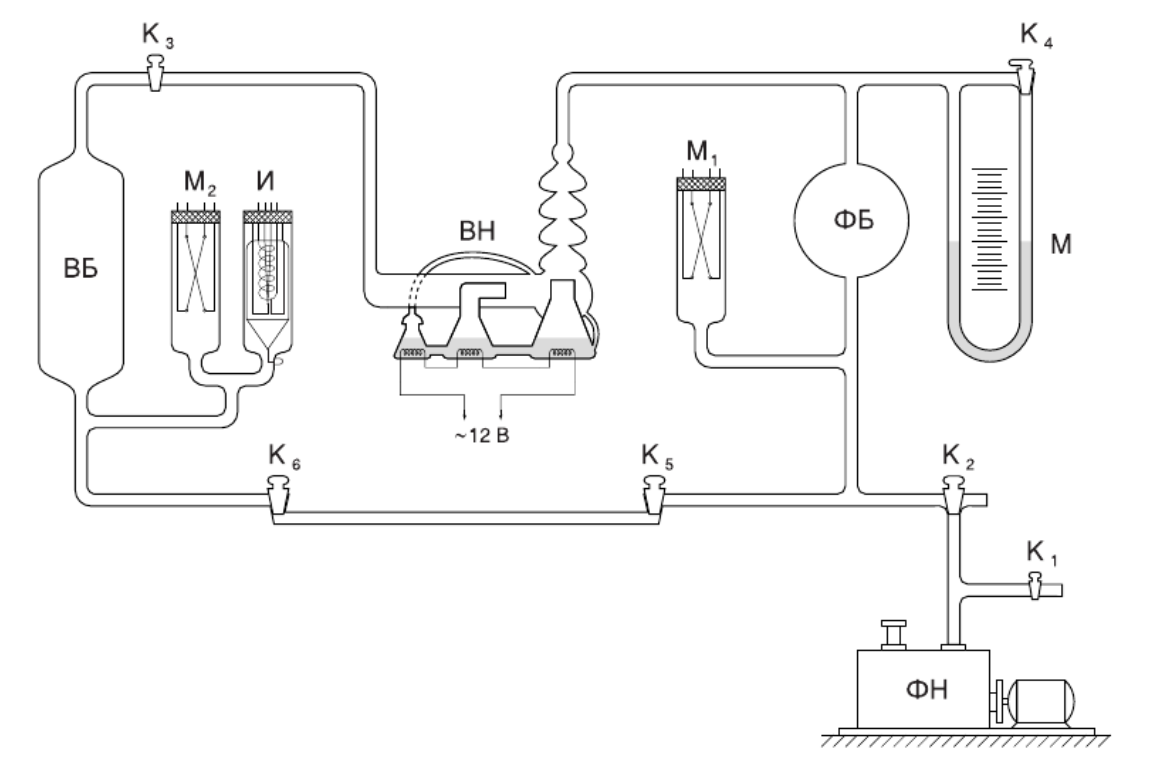
\includegraphics[width = 150mm]{apparatus.png}
	\caption{Экспериментальная установка}
\end{figure}
\paragraph{Параметры установки и начальные условия}
$$ V_\text{кап} = (50 \pm 3)~\text{см}^3, \quad
L_\text{кап} = 63~\text{мм}, \quad
d_\text{кап} = 0.9~\text{мм}, \quad
P_0 = 98 150~\text{Па}, \quad
\rho_\text{м} = 0.885~\text{г}/\text{см}^3 $$
\paragraph{Определение объёма форвакуумной и высоковакуумной частей установки}
\begin{enumerate}
	\item Открыть все краны, кроме K$_1$ и K$_2$.
\item Впустить в установку атмосферный воздух.
\item Закрыть K$_5$ и K$_6$, заперев в капилляре воздух.
\item Откачать установку формвакуумным насосом до $4 \cdot 10^{-4}$ торр.
\item Отсоединить вакуумный насос от установки, выключить его, подать на него атмосферу.
\item Закрыть K$_3$, отделив форвакуумную часть от высоковакуумной.
\item Закрыть K$_4$, приведя в готовность масляный манометр.
\item Открыть K$_5$.
\item Измерить давление масляным манометром $\Delta h_\text{ФВ} = (31.0 - 15.8)$ см масл. ст.  
\item Открыть K$_3$.
\item Измерить давление масляным манометром $\Delta h_\text{П} = (28.4 - 18.3)$ см масл. ст.
\item Открыть K$_4$.
\end{enumerate}
\paragraph{Получение высокого вакуума и измерение скорости откачки}
\begin{enumerate}
	\item Оставить установку без запертых частей, откачать форвакуумным насосом.
	\item Включить термопарные вакуумметры.
	\item Когда давление упало до $\mathbf{P_1 = 7 \cdot 10^{-3}\,\text{торр},}$ закрыть K$_6$.
	\item Включить нагреватель диффузионного насоса и подождать 10 минут.
	\item Включить ионизационный манометр.
	\item Измерить предельное давление в системе $\mathbf{P_\text{пр} = 72 \cdot 10^{-6}\,\text{торр}.}$
	\item Измерить скорость откачки:
	- отключить откачку краном K$_3$ и подождать, пока вакуум достаточно ухудшится ($10^{-3}$ торр),
	- открыть K$_3$ и фиксировать изменение показаний манометра со временем\*.
	\item Измерить величину потока $Q_\text{н}$: пе`рекрыть K$_3$ и фиксировать изменение показаний со временем.
	\item Повторить измерения пп. 7–8.
	\item Открыть K$_6$, дождаться установления давления: $\mathbf{P_\text{уст} = 1.4 \cdot 10^{-4}\,\text{торр}.}$
	\item Выключить установку.	\\
\textit{	* – фиксация зависимостей производилась при помощи видеосъёмки.}
\end{enumerate}

\paragraph{Обработка результатов}
\paragraph{Объёмы}
$$ V_\text{ФВ} = V_\text{кап} \frac{P_0}{\rho_\text{м}g \Delta h_\text{ФВ}} = 3.7\,\text{л},$$ 
Объём высоковакуумной части равен разности объёмов обеих частей и форвакуумной части: $V=V_\text{кап} - V_\text{ФВ}$\\
$$V_\text{ВВ} = V_\text{кап} \frac{P_0}{\rho_\text{м}g} \left( \frac{1}{\Delta h_\text{П}} - \frac{1}{\Delta h_\text{ФВ}} \right) = 1.9\,\text{л}$$\\	
\paragraph{Ухудшение вакуума}
Из паспорта вакуумметра ВИТ-2 узнали, что для перевода из мкА в торры надо полученное значение домножить на 100.
\begin{table}[H]
	\centering
	\caption{Данные полученные при улучшении вакуума}
	\begin{tabular}{c c c| c c c}
		\toprule
		$t$, c & $I_1\cdot10^{-1}$, мкА & $I_2\cdot10^{-1}$, мкА & $P\cdot10^{-5}$, торр & $(P-P_\text{пр})\cdot10^{-5}$, торр & $ln(P-P_\text{пр})$ \\ \midrule
		0    & 78                     & 74                     & 76                  & 68,8                              & 4,23                 \\ 
		1    & 62                     & 58                     & 60                  & 52,8                              & 3,97                 \\ 
		2    & 50                     & 53                     & 51,5                & 44,3                              & 3,79                 \\ 
		3    & 38                     & 41                     & 39,5                & 32,3                              & 3,48                 \\ 
		4    & 30                     & 33                     & 31,5                & 24,3                              & 3,19                 \\ 
		5    & 24                    & 26                     & 25                  & 17,8                              & 2,88                 \\ 
		6    & 22                     & 25                     & 23,5                & 16,3                              & 2,79                 \\ 
		7    & 18                     & 19                     & 18,5                & 11,3                              & 2,42                 \\ 
		8    & 16                     & 17                     & 16,5                & 9,3                               & 2,23                 \\ 
		9    & 12                     & 12                     & 12                  & 4,8                               & 1,57                 \\ \bottomrule
		\end{tabular}
		\end{table}
По полученным данным построим график зависимости $\ln(P-P_\text{пр})$ от $t$
\begin{figure}[H]
	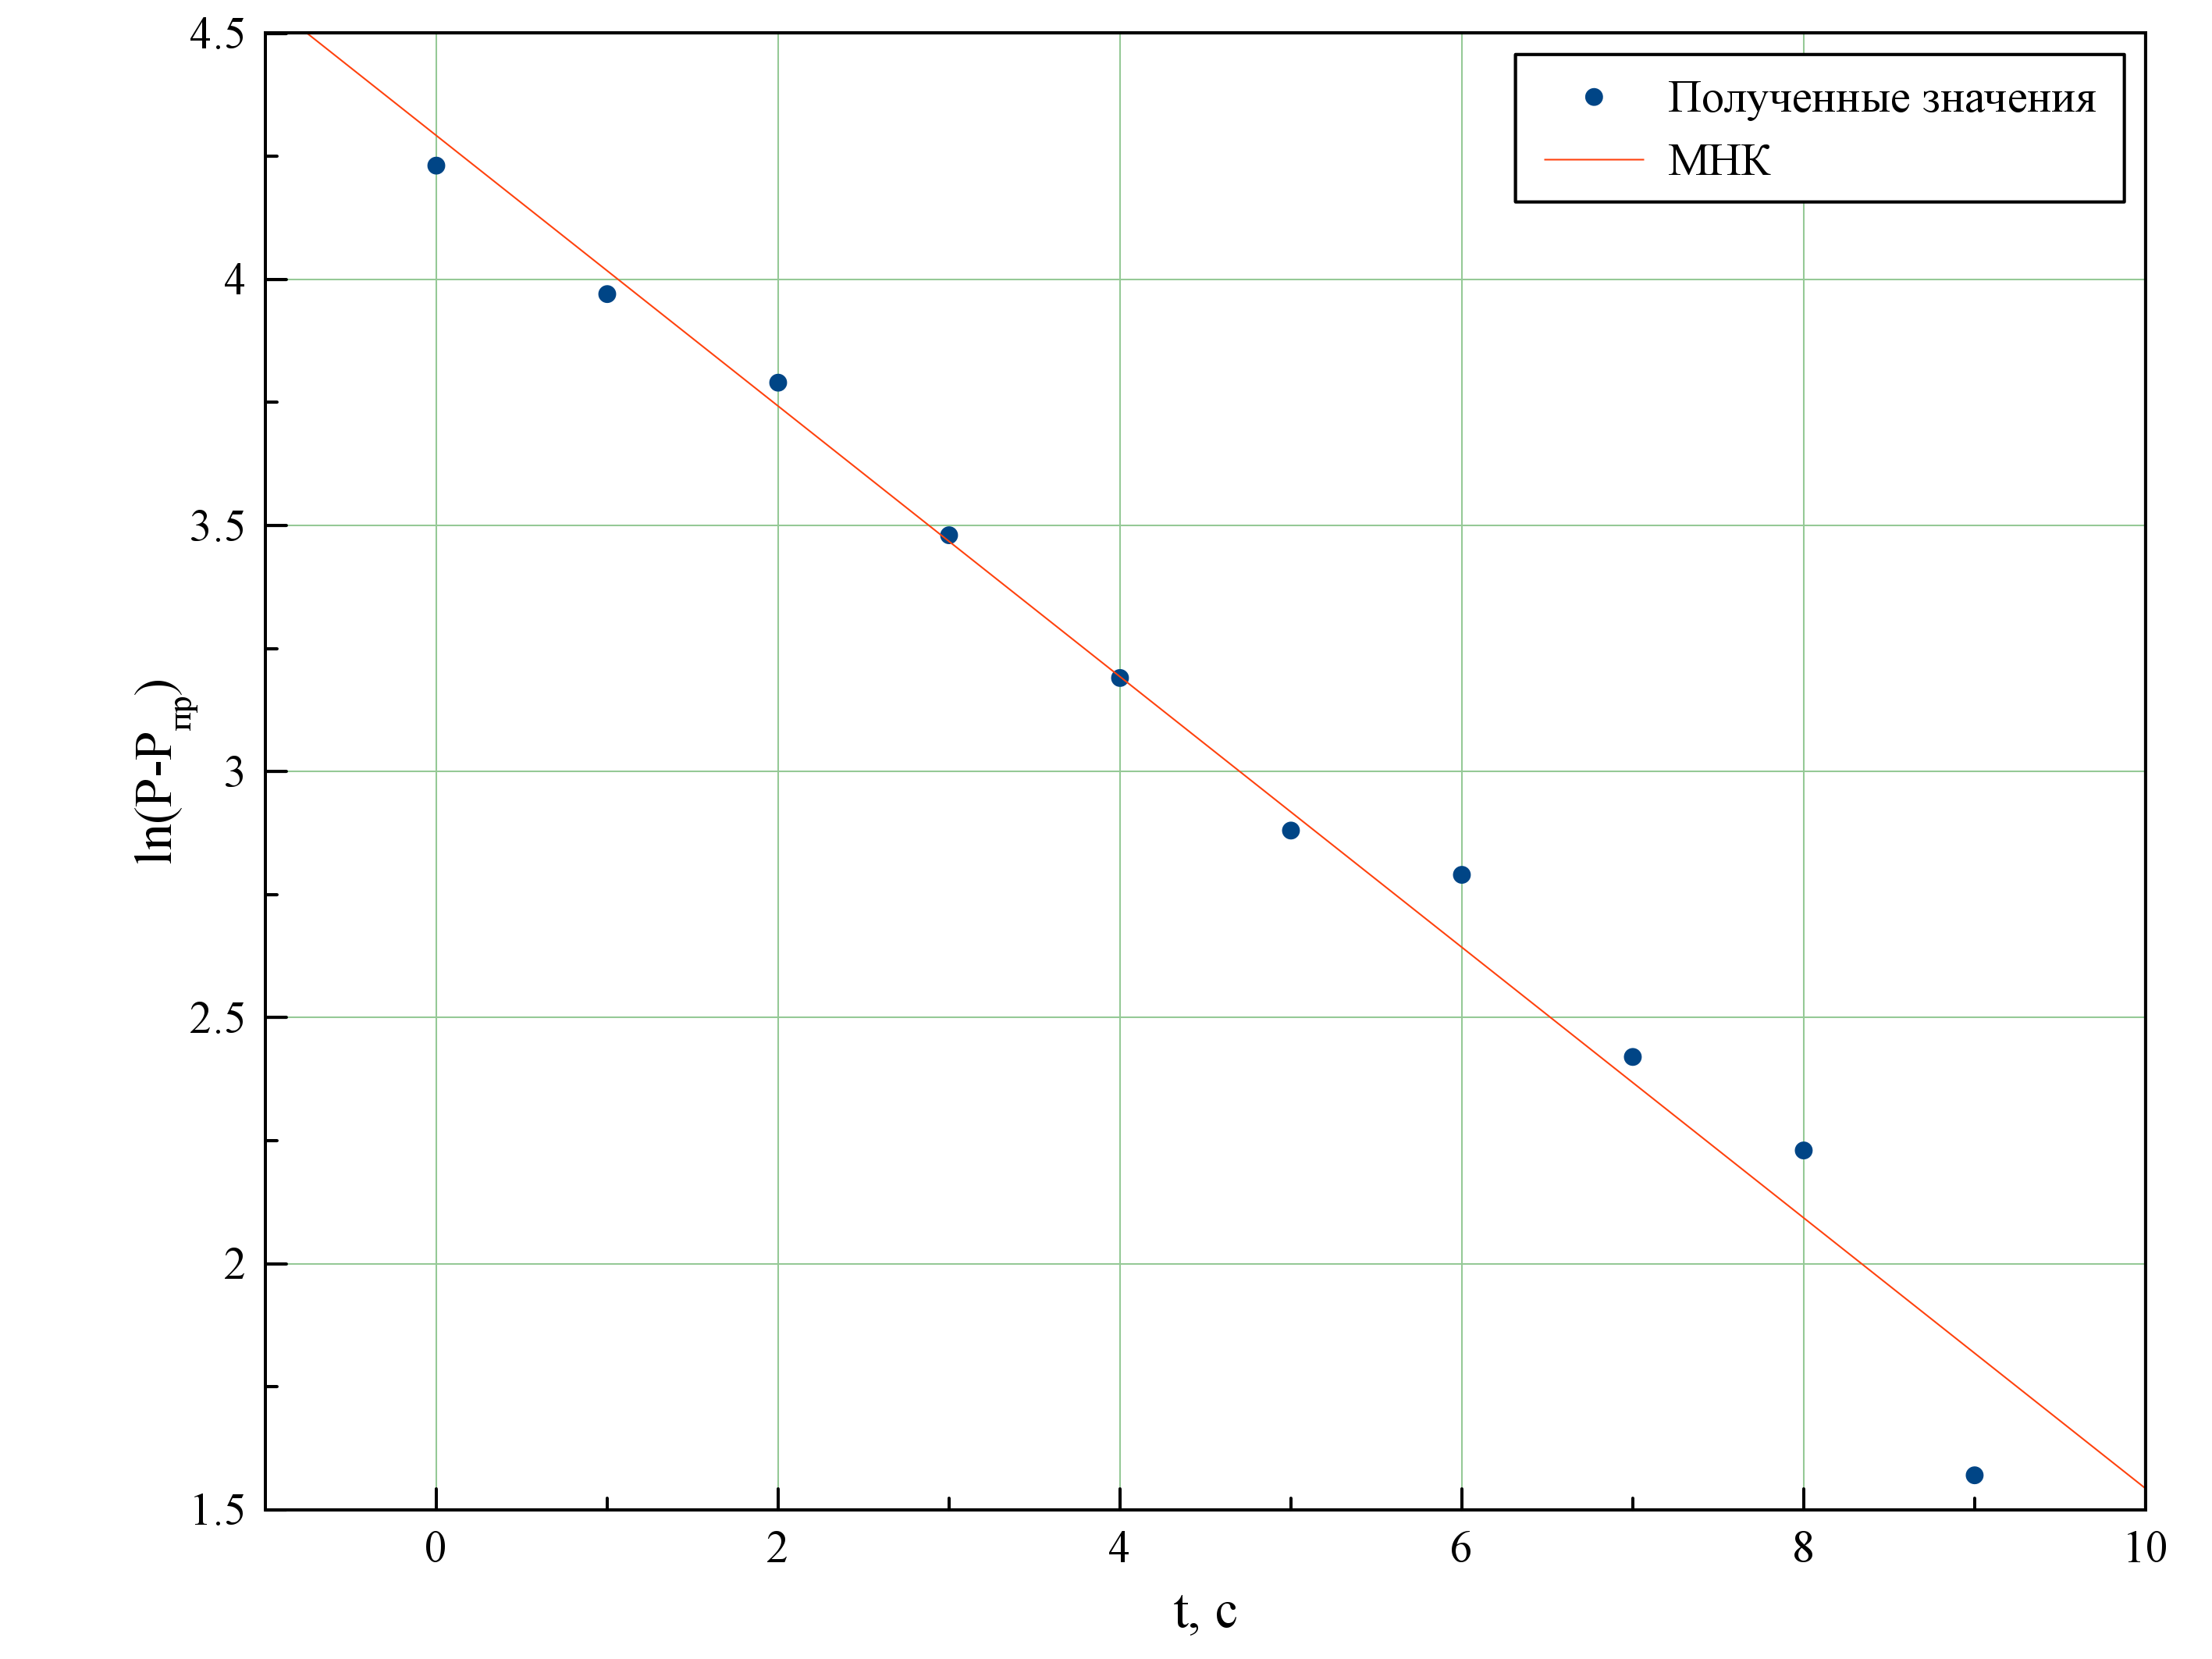
\includegraphics[width=150mm]{Graph1.png}
	\caption{График при улучшении вакуума}
\end{figure}
Посчитав с помощью МНК угловой коэффициент, получим $k = -2.7\pm0.1\cdot 10^{-1}$\\
Из уравнения (4) ясно, что $W = -k \cdot V_\text{вв} = 0.51 \pm 0.017 \,\dfrac{\text{л}}{\text{с}}$
\paragraph{Улучшение вакуума}
Теперь оценим величину потока $Q_\text{н}$
\begin{table}[H]
	\centering
	\caption{Данные полученные при ухудшении вакуума}
	\begin{tabular}{ccc|c}
		\toprule
		$t$, c & $I_1\cdot10^{-1}$, мкА & $I_2\cdot10^{-1}$, мкА & $P\cdot10^{-5}$, торр  \\ \midrule 
		0    & 22    & 22 & 22                      \\
		5    & 26    & 25 & 25,5                        \\
		10   & 30    & 30 & 30                         \\
		15   & 34    & 34 & 34                       \\
		20   & 38    & 39 & 38,5                     \\
		25   & 44    & 44 & 44                       \\
		30   & 48    & 47 & 47,5                  \\
		35   & 52    & 53 & 52,5                   \\
		40   & 56    & 56 & 56                     \\
		45   & 60    & 60 & 60                      \\
		50   & 64    & 65 & 64,5                    \\
		55   & 68    & 68 & 68                       \\
		60   & 72    & 72 & 72                     \\
		65   & 76    & 75 & 75,5                 \\ \bottomrule 
	\end{tabular}
\end{table}
По полученным данным построим график зависимости $P$ от $t$
\begin{figure}[H]
	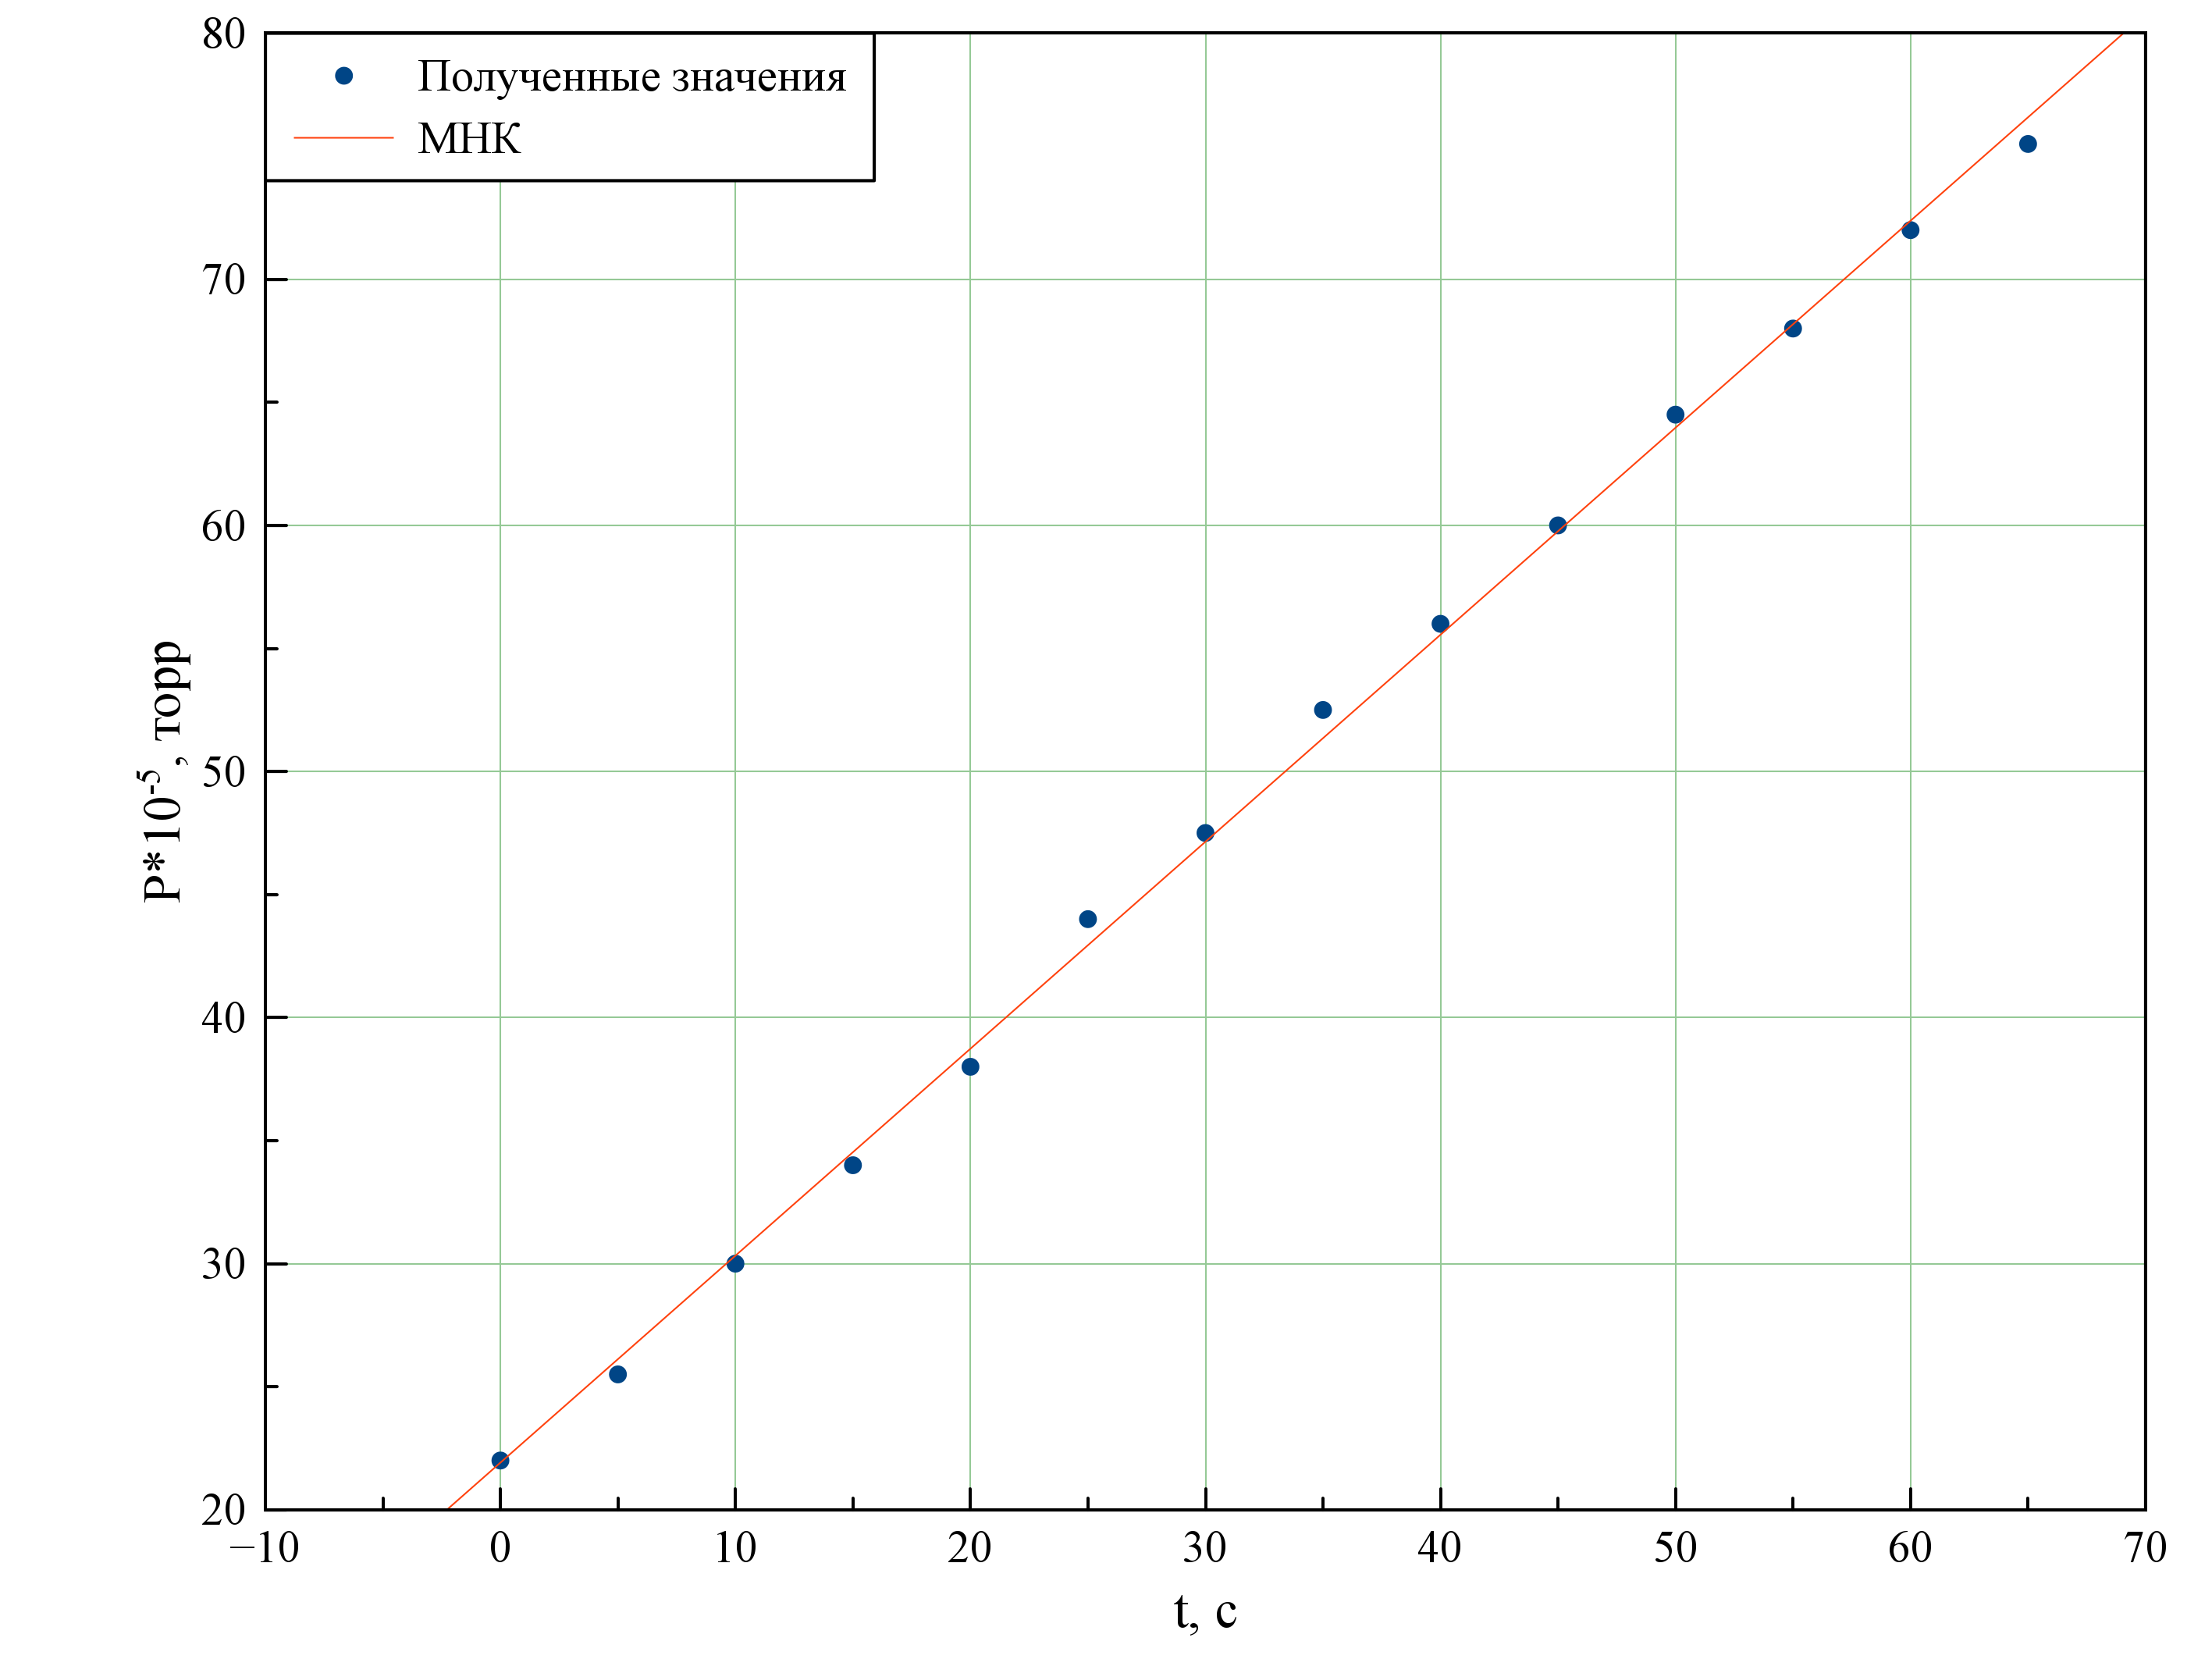
\includegraphics[width=150mm]{Graph2.png}
	\caption{График при улучшении вакуума}
\end{figure}
Посчитав с помощью МНК угловой коэффициент, получим $k = 8.4\pm0.01 \cdot 10^{-6} \,\dfrac{\text{торр}}{\text{с}}$\\
Мы знаем, что в этому случае(без откачки) изменение давления во времени описывается уравнением (1). Тогда $Q_\text{д} + Q_\text{и} = kV_\text{вв}$. Также $Q_\text{н}=P_\text{пр}W-Q_\text{д}-Q_\text{и}$\\ Значит $Q_\text{н}=P_\text{пр}W-kV_\text{вв} = 2.1 \cdot 10^{-5} \dfrac{\text{торр}\cdot\text{м}^3}{\text{с}}$, а $\sigma_{Q_\text{н}}=Q_\text{н}\sqrt{\varepsilon_k^2+\varepsilon_W^2} = 0.1\cdot 10^{-5} \dfrac{\text{торр}\cdot\text{м}^3}{\text{с}}$\\
\large
В итоге $Q_\text{н} = 2.1 \pm 0.1 \cdot 10^{-5} \dfrac{\text{торр}\cdot\text{м}^3}{\text{с}}$
\normalsize 
\paragraph{Производительность насоса} Рассчитаем производительность насоса по различию $P_\text{уст}$ и $P_\text{пр}$. Для этого используем формулу течения газа через трубу:
\begin{equation}
\dfrac{d(PV)}{dt}=\dfrac{4}{3}r^3\sqrt{\dfrac{2\pi RT}{\mu}}\dfrac{P_\text{ФВ}-P_\text{уст}}{L}
\end{equation}
Запишем формулу (2) для случаев, когда капилляр перекрыт и когда он открыт:
\begin{equation}
P_\text{пр}W = Q_1,\, P_\text{уст}=Q_1 + \dfrac{d(PV)_\text{капилл}}{dt} 
\end{equation}
$Q_1$ --- сумма всех натеканий, исключив её найдем $W$:
\begin{equation}
W = \dfrac{4}{3}r^3\sqrt{\dfrac{2\pi RT}{\mu}}\dfrac{P_\text{ФВ}-P_\text{уст}}{(P_\text{уст}-P_\text{пр})L}=0.41\,\dfrac{\text{л}}{\text{с}}
\end{equation}
\paragraph{Подведение итогов}
Были измерены объёмы форвакуумной и высоковакуумной частей установки: $V_\text{ФВ}=3.7\,\text{м}^3,\, V_\text{вв}=1.9\,\text{м}^3$. Была рассчитана скорость откачки системы $W$ двумя способами, при это полученные данные близки $W_\text{ухуд.} = 0.41\, \dfrac{\text{л}}{\text{с}}$, $W_\text{улучш.} = 0.51\, \dfrac{\text{л}}{\text{с}}$
\end{document}
